%%% LaTeX Template
%%% This template can be used for both articles and reports.
%%%
%%% Copyright: http://www.howtotex.com/
%%% Date: February 2011

%%% Preamble
\documentclass[paper=a4, fontsize=11pt]{scrartcl}	% Article class of KOMA-script with 11pt font and a4 format


\usepackage[italian]{babel}															% English language/hyphenation
\usepackage[protrusion=true,expansion=true]{microtype}				% Better typography
\usepackage{amsmath,amsfonts,amsthm}										% Math packages
\usepackage[pdftex]{graphicx}														% Enable pdflatex
%\usepackage{color,transparent}													% If you use color and/or transparency
\usepackage[hang, small,labelfont=bf,up,textfont=it,up]{caption}	% Custom captions under/above floats
\usepackage{epstopdf}																	% Converts .eps to .pdf
\usepackage{subfig}																		% Subfigures
\usepackage{booktabs}																	% Nicer tables
\usepackage[utf8x]{inputenc} 
\usepackage{listings}
\usepackage{xcolor}
\lstdefinestyle{sharpc}{language=[Sharp]C, frame=lr, rulecolor=\color{blue!80!black}}

  \usepackage{courier}

%%% Advanced verbatim environment
\usepackage{verbatim}
\usepackage{fancyvrb}
\DefineShortVerb{\|}								% delimiter to display inline verbatim text


%%% Custom sectioning (sectsty package)
\usepackage{sectsty}								% Custom sectioning (see below)
\allsectionsfont{%									% Change font of al section commands
	\usefont{OT1}{bch}{b}{n}%					% bch-b-n: CharterBT-Bold font
%	\hspace{15pt}%									% Uncomment for indentation
	}

\sectionfont{%										% Change font of \section command
	\usefont{OT1}{bch}{b}{n}%					% bch-b-n: CharterBT-Bold font
	\sectionrule{0pt}{0pt}{-5pt}{0.8pt}%	% Horizontal rule below section
	}


%%% Custom headers/footers (fancyhdr package)
\usepackage{fancyhdr}
\pagestyle{fancyplain}
\fancyhead{}														% No page header
\fancyfoot[C]{\thepage}										% Pagenumbering at center of footer
\renewcommand{\headrulewidth}{0pt}				% Remove header underlines
\renewcommand{\footrulewidth}{0pt}				% Remove footer underlines
\setlength{\headheight}{13.6pt}

%%% Equation and float numbering
\numberwithin{equation}{section}															% Equationnumbering: section.eq#
\numberwithin{figure}{section}																% Figurenumbering: section.fig#
\numberwithin{table}{section}																% Tablenumbering: section.tab#


\definecolor{pblue}{rgb}{0.13,0.13,1}
\definecolor{pgreen}{rgb}{0,0.5,0}
\definecolor{pred}{rgb}{0.9,0,0}
\definecolor{pgrey}{rgb}{0.46,0.45,0.48}


\usepackage{color}
\usepackage{xcolor}
\usepackage{listings}

 \lstset{
         basicstyle=\footnotesize\ttfamily, % Standardschrift
         %numbers=left,               % Ort der Zeilennummern
         numberstyle=\tiny,          % Stil der Zeilennummern
         %stepnumber=2,               % Abstand zwischen den Zeilennummern
         numbersep=5pt,              % Abstand der Nummern zum Text
         tabsize=2,                  % Groesse von Tabs
         extendedchars=true,         %
         breaklines=true,            % Zeilen werden Umgebrochen
         keywordstyle=\color{red},
    		frame=b,         
 %        keywordstyle=[1]\textbf,    % Stil der Keywords
 %        keywordstyle=[2]\textbf,    %
 %        keywordstyle=[3]\textbf,    %
 %        keywordstyle=[4]\textbf,   \sqrt{\sqrt{}} %
         stringstyle=\color{white}\ttfamily, % Farbe der String
         showspaces=false,           % Leerzeichen anzeigen ?
         showtabs=false,             % Tabs anzeigen ?
         xleftmargin=17pt,
         framexleftmargin=17pt,
         framexrightmargin=5pt,
         framexbottommargin=4pt,
         %backgroundcolor=\color{lightgray},
         showstringspaces=false      % Leerzeichen in Strings anzeigen ?        
 }
\lstloadlanguages{% Check Dokumentation for further languages ...
         %[Visual]Basic
         %Pascal
         %C
         %C++
         %XML
         %HTML
         %Java
{[Sharp]C}
 }
\usepackage{caption}
\DeclareCaptionFont{white}{\color{white}}
\DeclareCaptionFormat{listing}{\colorbox{gray}{\parbox{\textwidth}{#1#2#3}}}
\captionsetup[lstlisting]{format=listing,labelfont=white,textfont=white}

%%% Title	
\title{ \vspace{-1in} 	\usefont{OT1}{bch}{b}{n}
		\huge \strut Implementazione di Finding Triangles con Hadoop MapReduce\strut \\
		\Large \bfseries \strut Sistemi di elaborazione di grandi quantità di dati 2016 \strut
}
\author{ 									\usefont{OT1}{bch}{m}{n}
        Nicola Febbrari\\		\usefont{OT1}{bch}{m}{n}
        Università degli Studi di Verona\\	\usefont{OT1}{bch}{m}{n}
        Facoltà di Scienze\\
        \texttt{nicola.febbrari@studenti.univr.it}
}
\date{3 maggio 2017}

%%% Begin document
\begin{document}
\maketitle
\section{Introduzione}
Lo scopo del progetto è quello di implementare un algoritmo per calcolare il numero di triangoli presenti in un grafo non diretto, utilizzando le tecniche di MapReduce e il Framework Haddop.


\section{Il problema}
I social network negli ultimi anni hanno avuto una notevole diffusione, l'aumento del numero di utenti che interagistcono con questi sistemi ha avuto come conseguenza un  incremento della quantità di dati che devono essere registrati, gestiti ed ovviamente elaborati.\\
Un social network può essere rappresentato matematicamente da un grafo e una caratteristica molto interessante di questo grafo è il numero di triangoli\footnote{Dati 3 nodi (A,B,C) in un grafo, se un nodo A si relaziona sia con B che con C, nel grafo viene a formarsi un triangolo se esiste anche la relazione che lega B con C.} 
contenuti in sesso. Questo numero rapportato al totale dei triangoli che esisterebbero con una distribuzione casuale e uniforme delle relazioni può essere un indice di quanto sia social il grafo analizzato.\\
Gli algoritmi sviluppati prendono in considerazioni grafi non diretti.\\
\section{Strumenti e Framework}
\paragraph{Infrastruttura}
Per semplicità e rapidità di configurazione ho deciso di utilizzare Claudera come distribuzione di Hadoop nella sua versione per Docker.
\paragraph{Sviluppo}
Dovendo utilizzare il Framework Hadoop è il programma è stato scritto in Java utilizzando le API di Hadoop 2.6 Come IDE di sviluppo ho utilizzato è IntelliJ.  

\paragraph{Versioning}
Come sistema di versioning ho utilizzato Git e GitHub come spazio di hosting dei sorgenti.


\section{Implementazioni}
\subsection{Algoritmo 2 Jobs}
L'algoritmo a 2 Jobs prevede un prima fase in cui vengono elaborate tutte le relazioni e viene creata in output la combinazione di tutti i possibili triangoli a meno dell'ultimo arco necessario per chiudere il triangolo.\footnote{L'arco mancante è quello fra i 2 nodi maggiori del triangolo dove la relazione d'ordine del nodo è data dall'identificativo del nodo stesso} \\


\begin{figure}[h]
\centering
        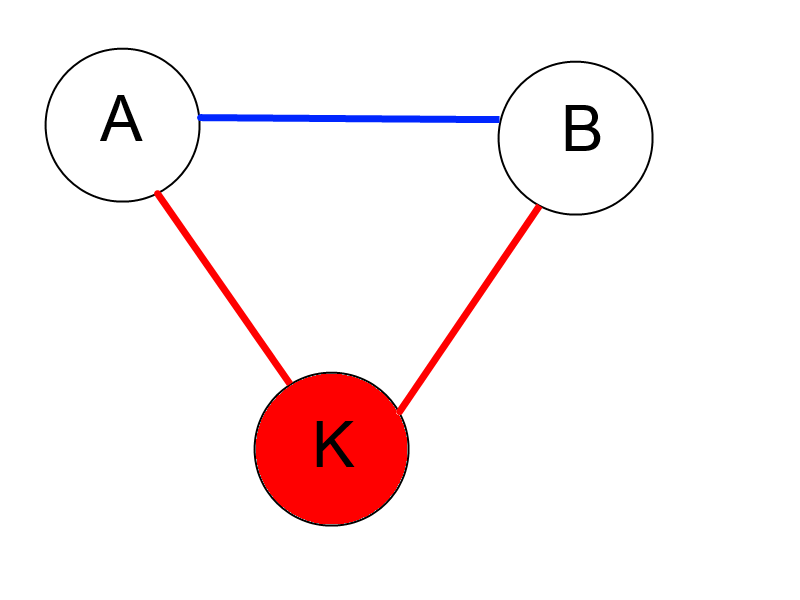
\includegraphics[totalheight=6cm]{Graph1.png}
    \caption{Il Job 1 elabora le relazioni rosse in cui K è il nodo minore del triangolo. Il Job2 cerca la relazione blu A B.}
    \label{fig:verticalcell} 
\end{figure}
\paragraph{Job1 Mapper}
Il grafo da analizzare è rappresentato da un file di testo in cui ogni nodo è identificato da un numero intero e ogni riga rappresenta la relazione fra due nodi.\\
Il mapper del primo Job carica il grafo e per ogni relazione contenuta in esso emette in output una copia \textit{chiave-valore} in cui la chiave è il nodo minore e il valore è il nodo maggiore.

\paragraph{Job1 GroupComparator}
Il GroupComparator raggruppa tutte le coppie generate dal mapper e per ogni possibile chiave crea una lista con i valori delle coppie aventi la stessa chiave
\paragraph{Job1 Reducer}

Il Redoucer elabora l'input raggruppato dal GroupComparator e, per ogni valore in cui K è chiave, costruisce una lista \textit{list} in cui aggiunge tutti i valori prodotti dal Mapper abbinati a K.\\
Quando la costruzione di \textit{list} è terminata e tutti i valori abbinati alla chiave K sono stati inseriti esegue il processo di scrittura dell'output delle coppie \textit{chiave-valore} in cui le chiavi sono date dalla combinazione di tutte le possibili coppie di valori presenti in \textit{list}, mentre il valore è il nodo K.

\paragraph{Job2 Mapper}
Il Mapper del secondo Job unisce l'outut del primo Job al grafo iniziale. Se l'elemento in INPUT A-B è una relazione di quelle presenti nel grafo iniziale, scrive in output un elemento \textit{chiave-valore} con una chiave strutturata (A-B,false) e come valore 0, se invece l'input è una coppia \textit{chiave-valore} (A-B)-K generata dal Job 1, scrive in output un elemento con chiave (A,B,true) e valore K.
\paragraph{Job2 GroupComparator}
Il secondo GroupComparator raggruppa tutti gli elementi generati dal Mapper mettendo insieme quelli che hanno la stessa prima parte di chiave (A-B) indipendentemente dal valore booleano che viene utilizzato solo per l'ordinamento degli elementi da sottoporre al Redoucer.

\paragraph{Job2 Reducer}
Il secondo Redoucer per ogni iterazione analizza una chiave (A-B) che raggruppa i valori sia di (A-B,false) che di (A-B,true). Se come primo elemento trova un (A-B,false) allora tutti i valori successivi positivi sono nodi che chiudono un trianogolo. Se invece il primo nodo analizzato ha chiave (A,B,true) allora l'iterazione del gruppo (A,B) puo' essere completamente saltata.
\subsection{Algoritmo 4 Jobs}
L'algoritmo a 4 Jobs prevede prima una fase in cui i primi 2 Jobs costuiscono una struttura dati che poi verrà usata negli ultimi 2 Jobs, i quali andranno ad eseguire il calcolo dei triangoli.
\paragraph{Job 1}
Il primo Job è molto semplice e per ogni arco emette un valore 1. Il redoucer conta tutti questi valori, ne fa la somma che poi scrive come output, questo valore rappresenta la quantità di nodi presenti nel grafo.
\paragraph{Job 2}
Il Mapper del secondo Job per ogni relazione A-B emette 2 valori A-1 e B-1, uno per ogni nodo che compone A-B.\\
Le funzioni di grouping e il Partitioner mi garantiscono che tutti i valori di uno stesso nodo vengono accumulati nello stesso redoucer e nello stesso ciclo iterativo. Completato il ciclo scrive in output, per ogni nodo, la somma di tutti i valori emessi dal mapper. Questo valore rappresenta il grado del nodo.
\paragraph{Job 3}
Nella seconda fase viene eseguito l'algoritmo vero e proprio.\\
Obiettivo del Job 3 è di trovare tutti i triangoli che sono composti da nodi Heavy Hitter, ovvero con un grado maggiore di $\sqrt{} m$ dove m è il numero degli archi delgrafo.\\
Il mapper utilizzando il lavoro dei Jobs precedenti costruisce in memoria un indice con i gradi di ogni nodo e esclude dall'analisi tutti i nodi non HH.\\
Definita una relazione $\prec$ di ordinamento dei nodi in base al grado, si può assumere che ogni trinagolo sia formato da 3 nodi (x,y,z) i quali sono legati dalle 3 relazioni typeA (x,y) con x$\prec$y, typeB (x,z) con x$\prec$z e typeC (y,z) ocn y$\prec$z.\\
Ogni relazione presente nel grafo può essre una delle 3 che compongono il triangolo, quindi se R=(u,v) una relazione che appartiene ad un triangolo allora sarà di tipo A e quindi  il triangolo sarebbe (u,v,?) oppure tipo B con (u,?,v) o di tipo C con (?,u,v).\\
Il task di Map per sfruttare il parallelismo dei redoucer divide l'input in tante parti quante le possibili combinazioni in cui ogni relazione può essere utilizzata per completare un triangolo.\\
Per implementare questa suddivisione, viene definita una funzione di hash \textit{H} e un paramentro \textit{bucket} che indica quanti sono i possibili valori in output della funzione. In base a questo parametro ogni relazione di input R(x,y) viene distribuita in 3bk Reducers utilizzando la funzione \textit{H} e seguendo questo schema: (h(x),h(y),1$\leq$i$\leq$b) impotizzando che R sia di tipo A , (h(x),1$\leq$i$\leq$b,h(y)) se R fosse di tipo B e (1$\leq$i$\leq$b,h(x),h(y)) se R fosse di tipo C. Ogni relazione R viene inclusa in tutti i possibili Redoucer in cui potrebbe essere utilizzata per il completamento di un triangolo.
Il Redoucer, dopo una opportuna ridefinizione delle classi di Gruouping e Ordinamento, scorrere tutti gli elementi in input. L'ordinamento è definito in modo da analizzare, per ogni nodo \textit{A}, prima le possili relazioni di \textit{tipo A}, per ognuna di esse viene inserito il nodo destinazione \textit{B} in una Lista LAa. Successivamente vengono analizzate le relazioni di a di tipo \textit{B} con \textit{C} come nodo di destinazione, per ognuna di esse viene preso creata una Map in cui la chiave è la copia formata da ogni elemento di Laa e c e il valore è il nodo a.
L'analisi successiva della relazione di tipo C fra a e d, se nella Map esiste una chiave formata dalla coppia a,d con valore e allora nel grafo esisterà un triangolo e,a,d.
L'ordinamento con cui viene eseguita questa analisi consente di ottimizzare lo spazio di memoria utilizzato e ci garantisce che ogni triangolo viene rilevato solo una volta.
\paragraph{Job 4}
Il Job 4 è molto simile al Job3 l'unica differenze è che in questo caso si volgiono escludere tutti i triangoli di tipo HH.\\
Data una relazione x,y se x è HH x,y potrebbe appartenere ad un triangolo non HH se solo se x,y è di tipo C. Infatti per la relazione di ordinamento rel definita precedentemente dato il triangolo T1(x,y,?) in cui x,y è di tipo A, qualsiasi ? e y sarebbero maggiori di x e quidi T1 sarebbe HH, la stessa cosa se x,y fosse di tipo B.\\
Grazie a questa caratteristica il mapper esclude le relazioni di tipo A e B in cui x,y ha x HH.
Il Redoucer è lo stesso del Job4.
\section{Test}
\subsection{Grafo semplice} 
11 nodi\\
16 archi\\
7 triangoli
\subsection{California road network\protect\footnote{http://snap.stanford.edu/data/roadNet-CA.html}} 
1965206 nodi\\
2766607 archi\\
120676 triangoli
\subsection{Youtube social network\protect\footnote{http://snap.stanford.edu/data/com-Youtube.html}} 

1134890 nodi\\
2987624 archi\\
3056386 triangoli

\section{Valutazioni}
\paragraph{Algoritmo 2 Jobs}
Semplice ma ha evidenziato problemi analizzando grafi di grandi dimensioni. 
\paragraph{Algoritmo 4 Jobs}
Più complesso ottimizzato dal punto di vista del tempo, tuttavia presenta sempre dei problemi nell'utilizzo della memoria. Sicuramente è possibile fare delle ottimizzazioni utilizzando delle strutture dati di opportune.\\ 
Nella mia implementazione ho cercato di utilizzare le strutture dati che mi permettevano di avere tempi di accesso rapidi e che non utlizzassero troppa memoria. Purtroppo ho notato che eseuendo più volte il programma rimane allocata della memoria, questo mi fa presupporre che vi sono alcuni memory leak.\\

\section{Sviluppi futuri}
Oltre alle ottimizzazioni nell'utilizzo di strutture dati più performanti, mi sarebbe piaciuto generare come artefatto del processo un immagine dock pronta all'uso. Sarebbe interessante provare a fare un deploy per testare questo container in un ambiente cloud che supporta Docker.

\end{document}